\documentclass[12pt,tikz,border=5pt]{article}
\usepackage[margin=1in]{geometry}
\usepackage[spanish]{babel}
\decimalpoint
\usepackage{tikz}
\usepackage{subcaption}
\usetikzlibrary{babel} 
\usepackage{setspace}
\usepackage{natbib}   
\usepackage{hyperref}
\usepackage{enumitem}
\usepackage{amsmath}
\usepackage{amssymb} 
\usepackage{amsfonts}
\usepackage{amsthm}
\newtheorem{ejercicio}{Ejercicio}[section]

\doublespacing

\title{Cálculo Diferencial e Integral \\ Licenciatura en Ingeniería en Computación}
\author{Dr. Julian Bravo \\ M. en C. Edwin Pérez}
\date{\today}

\begin{document}

\maketitle

\section{Funciones}

Ejercicios tomados del libro de Cálculo de una Variable Trascendentes Tempranas 4ta Edición\citep{stewart2001calculo}.

\begin{ejercicio}
  Se da la gráfica de una función $f$ en la figura \ref{fig:ejercicio1p1}. \medskip

  \begin{figure}[h!]
      \begin{center}
          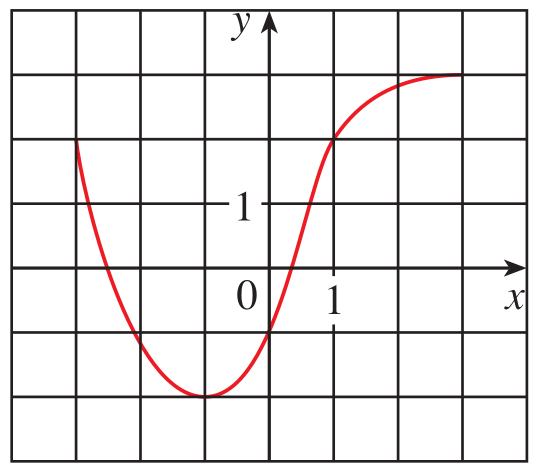
\includegraphics[width=0.30\textwidth]{figures/imagenEjercicio1p1.png}
      \end{center}
      \caption{Gráfica de una función $f$.}\label{fig:ejercicio1p1}
  \end{figure}

  \begin{enumerate}[label=(\alph*)]
    \item Establezca el valor de $f(-1)$.
      % El valor de $f(-1)=-2$.
    \item Estime el valor de $f(2)$.
      % El valor de $f(2)\approx2.9$.
    \item ¿Para cuáles valores de $x$ se tiene $f(x) = 2$?
      % Se buscan los puntos que tienen la forma $(x, 2)$ y de acuerdo a la figura \ref{fig:ejercicio1p1}, $x \in \{-3, 1\}$, es decir, $f(-3)=f(1)=2$.
    \item Estime los valores de $x$ tales que $f(x) = 0$.
      % Según la figura \ref{fig:ejercicio1p1}, $$f(x) = 0 \text{ cuando } x \approx -2.5 \text{ y } x \approx 0.25.$$
    \item Establezca el dominio y el rango de $f$.
      % El dominio de la función $f$ está dada por: $$Dom_{f} = \{x \in \mathbb{R} : -3\leq x \leq 3 \}.$$ También el dominio de $f$ se puede denotar como: $$Dom_{f}= [-3,3].$$
      % El rango de la función $f$ es:
      % \begin{align*}
      %   Im_{f} &= \{y \in \mathbb{R} : -2 \leq y \leq 3\} \\
      %   &= [-2,3].
      % \end{align*}
    \item ¿En qué intervalo es $f$ creciente?
      % Recuerde que $f$ es creciente en $[a,b]=I$ si para cualquier $x_{1}, x_{2} \in I$ donde $x_{1} < x_{2}$, se cumple que $f(x_{1}) < f(x_{2})$. De modo que al observar la figura \ref{fig:ejercicio1p1} se nota que $f$ crece en $[-1,3]$. \\
      % ¿En cúal intervalo $f$ es decreciente?
  \end{enumerate}
\end{ejercicio}

\begin{ejercicio}
  Se proporcionan las gráficas de $f$ y $g$ en la figura \ref{fig:ejercicio1p2}. \medskip

  \begin{figure}[h!]
      \begin{center}
          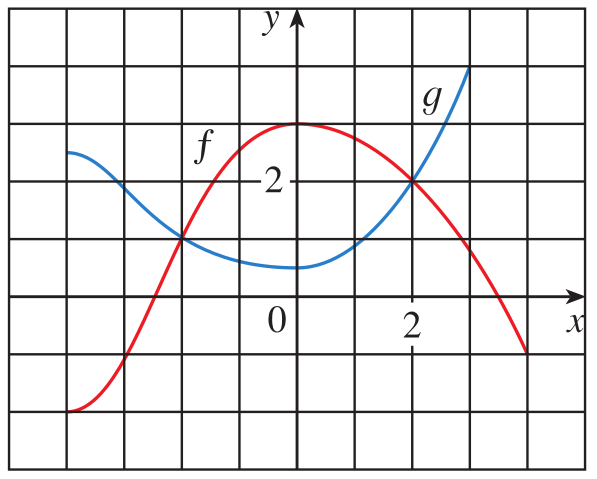
\includegraphics[width=0.30\textwidth]{figures/ejercicio1p2.png}
      \end{center}
      \caption{Gráficas de las funciones $f$ y $g$.}\label{fig:ejercicio1p2}
  \end{figure}

  \begin{enumerate}[label=(\alph*)]
    \item Dé los valores de $f(-4)$ y $g(3)$.
      % El valor de $f(-4)=-2$ y de $g(3)=4$.
    \item ¿Para cuáles valores de $x$ se tiene $f(x)=g(x)$?
      % Según la figura \ref{fig:ejercicio1p2} los puntos de intersección entre las curvas de $f$ y $g$ son $(-2,1)$ y $(2,2)$, entonces los valores de $x$ cuando $f(x)=g(x)$ son $x=-2$ y $x=2$.
    \item Estime la solución de la ecuación $f(x)=-1$.
      % La solución a la ecuación $f(x)=-1$ se puede deducir de la figura \ref{fig:ejercicio1p2} y está dada por: $$\{x \in \mathbb{R} : f(x)=-1 \} = \{-3,4\}$$ es decir $$f(-3)=f(4)=-1.$$
    \item ¿En qué intervalo $f$ es decreciente?
      % Por medio de la figura \ref{fig:ejercicio1p2} se deduce que $f$ es decreciente en $[0,4]$. ¿Sobre qué intervalo $f$ es decreciente? ¿Cuáles son los intervalos donde $g$ es creciente y decreciente?
    \item Establezca el dominio y el rango de $f$.
      % De acuerdo a la figura \ref{fig:ejercicio1p2}, el dominio de la función $f$ está dada por: $$Dom_{f} = \{x \in \mathbb{R} : -4\leq x \leq 4 \}$$  y la imagen de $f$ es: $$Im_{f} = \{y \in \mathbb{R} : -2 \leq y \leq 3\}.$$
    \item Establezca el dominio y el rango de $g$.
      % Al observar la figura \ref{fig:ejercicio1p2}, el dominio de la función $g$ está definida como: $$Dom_{g} = \{x \in \mathbb{R} : -4\leq x \leq 3 \},$$ mientras que el rango de $g$ es: $$Im_{g} = \{y \in \mathbb{R} : -2 \leq y \leq 0.5\}.$$
  \end{enumerate}
\end{ejercicio}

\begin{ejercicio}
  Determine si las curvas de la figura \ref{fig:ejercicio1p3} son una función de $x$. Si lo es, dé el dominio y el rango de la función.
  \begin{figure}[h!]
    \begin{center}
      \begin{subfigure}{0.2\textwidth}
          \centering
          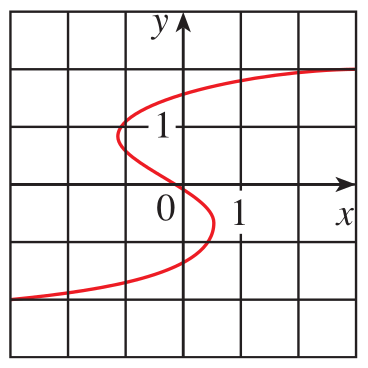
\includegraphics[width=\linewidth]{figures/ejercicio1p3pA.png}
          \caption{Gráfica $f$.}
          \label{fig:sub1}
      \end{subfigure}
      \hfill
      \begin{subfigure}{0.2\textwidth}
          \centering
          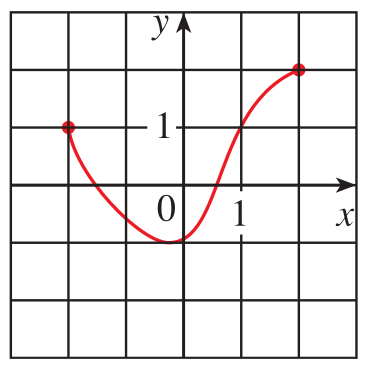
\includegraphics[width=\linewidth]{figures/ejercicio1p3pB.png}
          \caption{Gráfica $g$.}
          \label{fig:sub2}
      \end{subfigure}
      \hfill
      \begin{subfigure}{0.2\textwidth}
          \centering
          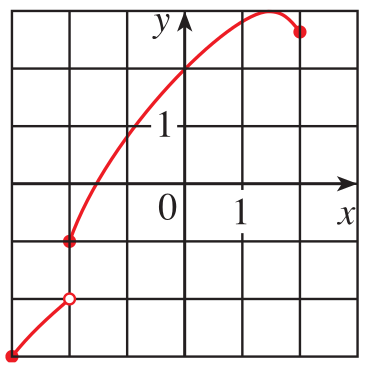
\includegraphics[width=\linewidth]{figures/ejercicio1p3pC.png}
          \caption{Gráfica $h$.}
          \label{fig:sub3}
      \end{subfigure}
      \hfill
      \begin{subfigure}{0.2\textwidth}
          \centering
          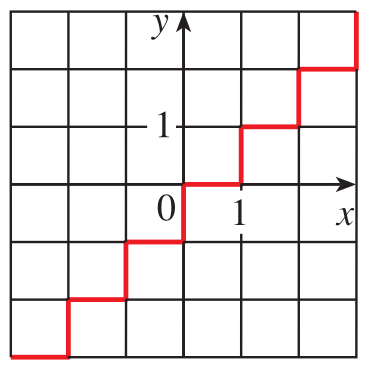
\includegraphics[width=\linewidth]{figures/ejercicio1p3pD.png}
          \caption{Gráfica $i$.}
          \label{fig:sub4}
      \end{subfigure}
    \end{center}
    \caption{Gráficas de las funciones $f$, $g$, $h$ e $i$.}\label{fig:ejercicio1p3}
  \end{figure}
\end{ejercicio}

\textbf{Tarea: ejercicios 9 y 10.}

\begin{ejercicio}
  Un globo esférico con radio $r$ pulgadas tiene el volumen $V(r) = \frac{4}{3} \pi r^{3}$. Encuentre una función que represente la cantidad de aire que se requiere para inflarlo desde un radio de $r$ pulgadas hasta otro de $r+1$ pulgadas.
\end{ejercicio}

\begin{ejercicio}
  Encuentre $f(2+h), \, f(x+h), \, \text{ y } \, \frac{f(x+h)-f(x)}{h}$, donde $h\neq0$. 
  \begin{enumerate}[label=(\alph*)]
    \item $f(x) = x - x^{2}$
    \item $f(x) = \frac{x}{x+1}$
  \end{enumerate}
\end{ejercicio}

\begin{ejercicio}
  Encuentre el dominio de la función.
  \begin{enumerate}[label=(\alph*)]
    \item $f(x) = \frac{x+2}{x^{2} - 1}$
    \item $f(x) = \frac{x^4}{x^2+x-6}$
    \item $g(x) = \sqrt[4]{x^2 - 6x}$
  \end{enumerate}
\end{ejercicio}

\textbf{Tarea: ejercicios 26 y 27}

\begin{ejercicio}
  Encuentre el dominio, la imagen y trace la gráfica de la función $h(x) = \sqrt{4 - x^2}$.
\end{ejercicio}

\begin{ejercicio}
  Encuentre el dominio y trace la gráfica de la función.
  \begin{enumerate}[label=(\alph*)]
    \item $g(x) = \sqrt{x - 5}$
    \item $g(x) = \sqrt{6 - 2x}$
    \item $G(x) = |x| + x$
    \item $f(x) = \frac{x}{|x|}$
    \item $f(x) = \frac{x^2 + 5x + 6}{x + 2}$
    \item $f(x) = 
      \begin{cases}
        -1, &\text{ si } x \leq -1\\
        3x + 2, &\text{ si } |x| < 1\\
        7 - 2x, &\text{ si } x \geq 1\\
      \end{cases}$
  \end{enumerate}
\end{ejercicio}

\textbf{Tarea: ejercicios 29, 30, 34, 37, 38, 39 y 41 - 46.}

\begin{ejercicio}
  Encuentre una fórmula para la función descrita y dé su dominio. 
  \begin{enumerate}[label=(\alph*)]
    \item Un rectángulo tiene un perímetro de $20\,m$. Exprese el área del rectángulo como función de la longitud de uno de sus lados.
    \item Un rectángulo tiene un área de $16\,m^2$. Exprese su perímetro como función de la longitud de uno de sus lados.
    \item Exprese el área de un triángulo equilátero como función de la longitud de uno de los lados.
    \item Exprese el área superficial de un cubo como función de su volumen.
    \item Una caja rectangular abierta, con volumen de $2\,m^3$, tiene una base cuadrada. Exprese el área superficial de la caja como función de la longitud de uno de los lados de la base.
  \end{enumerate}
\end{ejercicio}
\textbf{Tarea: ejercicios 52 - 54, 56, 57.}

\bibliographystyle{abbrv}
\bibliography{cite}

\end{document}
